\documentclass[10pt,letterpaper]{article}
%\usepackage{times}
\usepackage[margin=1in,hmargin=1in]{geometry}
\usepackage{amsmath}
\usepackage{tikz,url}
\usepackage{amssymb}
\usepackage{fancyhdr}
\usetikzlibrary{matrix}
\usepackage{listings}
\usepackage{tabularx}
\usepackage{xcolor}
\usepackage{graphicx}
\usepackage{graphics}
\usepackage{titling}
\pagestyle{fancy}
\usepackage{float}
\usepackage{fancyvrb}
\usepackage{verbatim}
\usepackage{enumitem}
\usepackage{alltt}
\usepackage{pdfpages}
\usepackage{multicol}
%\usepackage{float}
%\restylefloat{table}

\fancyhead[LO]{STAT W4201 Advanced Data Analysis}
\fancyhead[RO]{HW 7}
\fancyhead[LE]{STAT W4201 Advanced Data Analysis}
\fancyhead[RE]{HW 7}
\title{\textbf {Homework 7}}
\author{{Qianbo Wang}\\{uni: qw2180}}
\date{}
\setlength{\droptitle}{-5em}
\setlength{\parindent}{0pt}
\makeatletter
\newcommand{\rmnum}[1]{\romannumeral #1}
\newcommand{\Rmnum}[1]{\expandafter\@slowromancap\romannumeral #1@}
\makeatother
\lstset{
language=R,
tabsize=4, 
%frame=shadowbox, 
commentstyle=\color{red!50!green!50!blue!50},
%rulesepcolor=\color{red!20!green!20!blue!20},
keywordstyle=\color{blue!90},
showstringspaces=false,
stringstyle=\ttfamily, 
keepspaces=true, 
breakindent=22pt, 
numbers=none,
stepnumber=1,
numberstyle=\tiny, 
numberstyle={\color[RGB]{0,192,192}\tiny} ,
numbersep=5pt,  
basicstyle=\footnotesize, 
showspaces=false, 
flexiblecolumns=true, 
comment=[l]{\#},
texcl=true,
escapeinside={\$$}{\^^M},
breaklines=true, 
breakautoindent=true,
breakindent=4em, 
aboveskip=1em, 
tabsize=2,
showstringspaces=false, 
backgroundcolor=\color[RGB]{244,244,244},   
fontadjust,
captionpos=t,
framextopmargin=2pt,framexbottommargin=2pt,abovecaptionskip=-3pt,belowcaptionskip=3pt,
extendedchars=false,columns=flexible
}

\begin{document}
\maketitle
\thispagestyle{fancy}
\vspace{-2em}

\textbf{Consider the ChickWeight data in R. The body weights of the chicks were measured at birth (i.e., time=0) and every second day thereafter until day 20. They were also measured on day 21. There were four groups of chicks on different protein diets.}\\

\textbf{Categorize ‘weight’ as a binary variable, with Weight Group = 1 (or Low), if weight $>$ 215 mg, and 0, Otherwise.}

\section*{Problem 1}
\textbf{Consider comparing Diet Levels 1 and 4 on Day 21.}
\begin{enumerate}[leftmargin=0cm,itemindent=.5cm,labelwidth=\itemindent,labelsep=0cm,align=left]
\item[\textbf{(a).} ] \textbf{Determine whether there is association between Diet and Weight, using logistic regression, without adjusting for Birth Weight. Interpret what the estimated parameters denote.}

Construct a logistic regression model with adjusting for Birth Weight with Weight for Diet group 1 and 4 on day 21. Restructure the data as categorical data type. The response and explanatory variable is like:\\
\begin{multicols}{2}
\[\text{Weight}_i=  
\left \{
  \begin{tabular}{cc}
  1 &  $\text{Weight}>215$\\
  0 &  $\text{Weight} \leq 215$\\
  \end{tabular}
\right.
\]

\[\text{Group}_i=  
\left \{
  \begin{tabular}{cc}
  1 &  $\text{Diet}=1$\\
  0 &  $\text{Diet} \neq 1$ \\
  \end{tabular}
\right.
\]
\end{multicols}
Then the result is as follows:
\begin{center}
Logistic Regression without adjust result
\verbatiminput{log_day21.txt}
\end{center}
The model is:
\[\text{logit(p)} =0.2231-1.6895*\text{Group} \]
So for Diet group 1, the model is:
\[\text{logit(p)} = 0.2231-1.6895\]
And for Diet group 4, the model is:
\[\text{logit(p)} = 0.2231\]

There are two parameters here, intercept $\beta_0$, and coefficient $\beta_1$ on Diet group.
\begin{enumerate}[leftmargin=0cm,itemindent=.5cm,labelwidth=\itemindent,labelsep=0cm,align=left]
\item[\textbullet] $\beta_0$ denotes the log odds ratio of $\text{Weight}>215$ for Diet group 4, i.e., the odds ratio of $\text{Weight}>215$  for Diet group 4 is $e^0.2231$.
\item[\textbullet] $\beta_1$ denotes the log odds ratio of $\text{Weight}>215$ for Diet group 1 relative to Diet Group 4, i.e., odds ratio of $\text{Weight}>215$  for Diet group 1 relative to Diet Group 4 is $e^{-1.6895}$,
and also the odds ratio of $\text{Weight}>215$ for Diet group 1 is $e^{-1.4664}$.\\

Since $\text{p-value}$ for the intercept and Group are both $\text{p-value}>0.05$, so we don't reject the null, i.e., there are no significant association between Diet Group 1 and 4 and Categorical Weight without adjusting for BirthWeight.
\end{enumerate}

\item[\textbf{(b).} ] \textbf{Repeat (a) adjusting for Birth Weight. Interpret what the estimated parameters denote.}

Construct a logistic regression model without adjusting for Birth Weight with Weight for Diet group 1 and 4 on day 21. Restructure the data as categorical data type. The response and explanatory variable is like:\\
\begin{multicols}{2}
\[\text{Weight}_i=  
\left \{
  \begin{tabular}{cc}
  1 &  $\text{Weight}>215$\\
  0 &  $\text{Weight} \leq 215$\\
  \end{tabular}
\right.
\]

\[\text{Group}_i=  
\left \{
  \begin{tabular}{cc}
  1 & Diet $= 1$\\
  0 & Diet $= 4$ \\
  \end{tabular}
\right.
\]
\end{multicols}
Then the result is as follows:
\begin{center}
Logistic Regression with adjust result
\verbatiminput{log_day21_adjust.txt}
\end{center}
The model is:
\[ \text{logit(p)} = 57.2079-1.2935*\text{Group} -1.3899*\text{BirthWeight}\]
So for Diet group 1 the model is:
\[ \text{logit(p)} = 57.2079-1.2935-1.3899*\text{BirthWeight}\]
And for Diet group 4 the model is:
\[ \text{logit(p)} = 57.2079-1.3899*\text{BirthWeight}\]

There are three parameters here, intercept $\beta_0$, and coefficient $\beta_1$ on Diet group, and coefficient $\beta_2$ on BirthWeight. 
\begin{enumerate}[leftmargin=0cm,itemindent=.5cm,labelwidth=\itemindent,labelsep=0cm,align=left]
\item[\textbullet] $\beta_0$ denotes when BirthWeight is given 0, the log odds ratio of $\text{Weight}>215$ for Diet group 4, i.e., when BirthWeight=0(which is not realistic), the odds ratio of $\text{Weight}>215$ for Diet group 4 is $e^{57.2079}$, and the odds ratio of $\text{Weight}>215$ for Diet group 4 when given $\text{BirthWeight}=x$ is $e^{57.2079-1.3899x}$.
\item[\textbullet] $\beta_1$ denotes the log odds ratio of $\text{Weight}>215$ for Diet group 1 relative to Diet Group 4 when given BirthWeight = 0(which is not realistic), i.e., when $\text{BirthWeight}=0$ odds ratio of $\text{Weight}>215$ for Diet group 1 relative to Diet Group 4 is $e^{-1.3899}$, and odds ratio of $\text{Weight}>215$ for Diet group 1 when given $\text{BirthWeight}=x$ is $e^{55.9144-1.3899x}$
\item[\textbullet] $\beta_2$ denotes under same Diet Group, the change in log odds for $\text{Weight}>215$ when the BirthWeight is different, i.e., under same Diet Group, 1 unit change in BirthWeight will cause the odds for $\text{Weight}>215$ in day 21 change $e^{-1.3899}$.
\end{enumerate}
Since $\text{p-value}$ for the intercept, Group and BirthWeight are all $\text{p-value}>0.05$, so we don't reject the null, i.e., there are no significant association between Diet Group 1 and 4 and Categorical Weight with adjusting for BirthWeight. 
\end{enumerate}
\section*{Problem 2}
\textbf{Repeat 1 for all 4 Diet Levels.}
\begin{enumerate}[leftmargin=0cm,itemindent=.5cm,labelwidth=\itemindent,labelsep=0cm,align=left]
\item[\textbf{(a).} ] \textbf{Without adjusting for BirthWeight.}

Construct a logistic regression model without adjusting for Birth Weight with Weight for Diet group 1 and 4 on day 21. Restructure the data as categorical data type. The response and explanatory variable is like:\\
\begin{multicols}{2}
\[\text{Weight}_i=  
\left \{
  \begin{tabular}{cc}
  1 & $\text{Weight}>215$\\
  0 & $\text{Weight} \leq 215$ \\
  \end{tabular}
\right.
\]
\[\text{Group1}_i=  
\left \{
  \begin{tabular}{cc}
  1 &  $\text{Diet} = 1$\\
  0 &  $\text{Diet} \neq 1$\\
  \end{tabular}
\right.
\]

\[\text{Group2}_i=  
\left \{
  \begin{tabular}{cc}
  1 &  $\text{Diet} = 2$\\
  0 &  $\text{Diet} \neq 2$\\
  \end{tabular}
\right.
\]
\[\text{Group3}_i=  
\left \{
  \begin{tabular}{cc}
  1 &  $\text{Diet} = 3$\\
  0 &  $\text{Diet} \neq 3$ \\
  \end{tabular}
\right.
\]
\end{multicols}
Then the result is as follows:
\begin{center}
Logistic Regression without adjust result
\verbatiminput{log_day21_all.txt}
\end{center}
The model is:
\[ \text{logit(p)} = 0.2231-1.6895*\text{Group1}-0.2231*\text{Group2}+1.1632*\text{Group3}\]
So for Diet group 1, the model is:
\[ \text{logit(p)} = 0.2231-1.6895=-1.4664\]
And for Diet group 2, the model is:
\[\text{logit(p)} = 0.2231-0.2231=0\]
And for Diet group 3, the model is:
\[\text{logit(p)} = 0.2231+1.1632=1.3863\]
And for Diet group 4, the model is:
\[\text{logit(p)} = 0.2231\]

There are four parameters here, intercept $\beta_0$, and coefficient $\beta_1$ on Diet group1, coefficient $\beta_2$ on Diet group2, coefficient $\beta_3$ on Diet group3.
\begin{enumerate}[leftmargin=0cm,itemindent=.5cm,labelwidth=\itemindent,labelsep=0cm,align=left]
\item[\textbullet] $\beta_0$ denotes the log odds ratio of $\text{Weight}>215$ for Diet group 4, i.e., the odds ratio of $\text{Weight}>215$ for Diet group 4 is $e^{0.2231}$.
\item[\textbullet] $\beta_1$ denotes the log odds ratio of $\text{Weight}>215$ for Diet group 1 relative to Diet Group 4, i.e., odds ratio of $\text{Weight}>215$ for Diet group 1 relative to Diet Group 4 is $e^{-1.6895}$, and odds ratio of $\text{Weight}>215$ for Diet group 1 is $e^{-1.4664}$.
\item[\textbullet] $\beta_2$ denotes the log odds ratio of $\text{Weight}>215$ for Diet group 2 relative to Diet Group 4, i.e., odds ratio of $\text{Weight}>215$ for Diet group 2 relative to Diet Group 4 is $e^{-0.2231}$, and odds ratio of $\text{Weight}>215$ for Diet group 2 is $e^{0}=1$.
\item[\textbullet] $\beta_3$ denotes the log odds ratio of $\text{Weight}>215$ for Diet group 3 relative to Diet Group 4, i.e., odds ratio of $\text{Weight}>215$ for Diet group 3 relative to Diet Group 4 is $e^{1.1632}$, and odds ratio of $\text{Weight}>215$ for Diet group 3 is $e^{1.3863}$.\\

Since $\text{p-value}$ for the intercept, Group1, Group2, Group3 are all $\text{p-value}>0.05$, so we don't reject the null, i.e., there are no significant association between Diet Group from 1 to 4 and Categorical Weight without adjusting for BirthWeight. 
\end{enumerate}

\item[\textbf{(b).} ] \textbf{With adjusting for BirthWeight.}

Construct a logistic regression model without adjusting for Birth Weight with Weight for Diet group 1 and 4 on day 21. Restructure the data as categorical data type. The response and explanatory variable is like:\\
\begin{multicols}{2}
\[\text{Weight}_i=  
\left \{
  \begin{tabular}{cc}
  1 &  $\text{Weight}>215$\\
  0 &  $\text{Weight} \leq 215$\\
  \end{tabular}
\right.
\]
\[\text{Group1}_i=  
\left \{
  \begin{tabular}{cc}
  1 &  $\text{Diet}= 1$\\
  0 &  $\text{Diet}\neq 1$ \\
  \end{tabular}
\right.
\]

\[\text{Group2}_i=  
\left \{
  \begin{tabular}{cc}
  1 &  $\text{Diet}= 2$\\
  0 &  $\text{Diet} \neq 2$\\
  \end{tabular}
\right.
\]
\[\text{Group3}_i=  
\left \{
  \begin{tabular}{cc}
  1 &  $\text{Diet}= 3$\\
  0 &  $\text{Diet} \neq 3$\\
  \end{tabular}
\right.
\]
\end{multicols}

Then the result is as follows:
\begin{center}
Logistic Regression with adjust result
\verbatiminput{log_day21_all_adjust.txt}
\end{center}
The model is:
\[\text{logit(p)} = 26.3751-1.3805*\text{Group1}-0.3800*\text{Group2}+1.1864*\text{Group3}-0.6389*\text{BirthWeight}\]
So for Diet group 1 the model is:
\[\text{logit(p)} = 26.3751-1.3805-0.6389*\text{BirthWeight}\]
And for Diet group 2 the model is:
\[\text{logit(p)} = 26.3751-0.3800-0.6389*\text{BirthWeight}\]
And for Diet group 3 the model is:
\[\text{logit(p)} = 26.3751+1.1864-0.6389*\text{BirthWeight}\]
And for Diet group 4 the model is:
\[\text{logit(p)} = 26.3751-0.6389*\text{BirthWeight}\]

There are five parameters here, intercept $\beta_0$, and coefficient $\beta_1$ on Diet group1,  coefficient $\beta_2$ on Diet group2, coefficient $\beta_3$ on Diet group3, and coefficient $\beta_4$ on BirthWeight.

\begin{enumerate}[leftmargin=0cm,itemindent=.5cm,labelwidth=\itemindent,labelsep=0cm,align=left]
\item[\textbullet] $\beta_0$ denotes the log odds ratio of $\text{Weight}>215$ for Diet group 4 under given BirthWeight=0(which is not realistic), i.e., the odds ratio of $\text{Weight}>215$ for Diet group 4 when BirthWeight=0 is $e^{26.3751}$, and the odds ratio of $\text{Weight}>215$ for Diet group 4 under given $\text{BirthWeight}=x$ is $e^{26.3751-0.6389x}$.
\item[\textbullet] $\beta_1$ denotes the log odds ratio of $\text{Weight}>215$ for Diet group 1 relative to Diet Group 4, under given BirthWeight=0(which is not realistic), i.e., when BirthWeight=0, odds ratio of $\text{Weight}>215$ for Diet group 1 relative to Diet Group 4 is $e^{-1.3805}$, and under given $\text{BirthWeight}=x$ odds ratio of $\text{Weight}>215$ for Diet group 1 relative to Diet Group 4 is $e^{-1.3805-0.6389x}$.
\item[\textbullet] $\beta_2$ denotes the log odds ratio of $\text{Weight}>215$ for Diet group 2 relative to Diet Group 4, under given BirthWeight=0(which is not realistic), i.e., when BirthWeight=0, odds ratio of $\text{Weight}>215$ for Diet group 2 relative to Diet Group 4 is $e^{1.1864}$, and under given $\text{BirthWeight}=x$ odds ratio of $\text{Weight}>215$ for Diet group 2 relative to Diet Group 4 is $e^{1.1864-0.6389x}$.
\item[\textbullet] $\beta_3$ denotes the log odds ratio of $\text{Weight}>215$ for Diet group 3 relative to Diet Group 4, under given BirthWeight=0(which is not realistic), i.e., when BirthWeight=0, odds ratio of $\text{Weight}>215$ for Diet group 2 relative to Diet Group 4 is $e^{1.1864}$, and under given $\text{BirthWeight}=x$ odds ratio of $\text{Weight}>215$ for Diet group 3 relative to Diet Group 4 is $e^{1.1864-0.6389x}$.
\item[\textbullet] $\beta_4$ denotes under same Diet Group, the change in log odds for $\text{Weight}>215$ when the BirthWeight is changing, i.e., under same Diet Group, 1 unit change in BirthWeight will cause the odds for $\text{Weight}>215$ in day 21 change $e^{-0.6389}$.
\end{enumerate}
Since $\text{p-value}$ for the intercept, Group1, Group2, Group3 and BirthWeight are all $\text{p-value}>0.05$, so we don't reject the null, i.e., there are no significant association between Diet Group from 1 to 4 and Categorical Weight with adjusting for BirthWeight. 
\end{enumerate}

\section*{Problem 3}
\textbf{Repeat 1 using the L-1 regularized logistic regression.}

We should use BirthWeight and Group for L-1 logistic regression. The cross validation plot of choosing best gamma is as follows:
\begin{center}
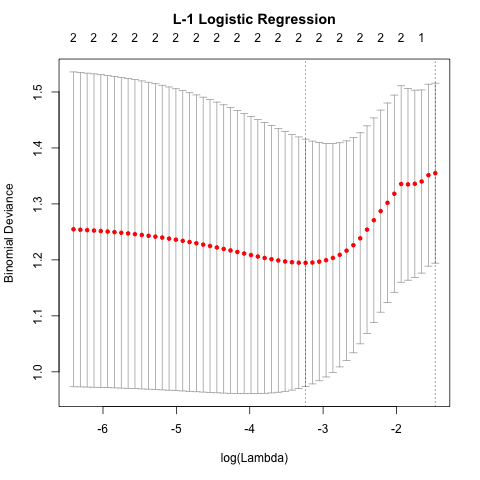
\includegraphics[scale=0.7]{cv_l1log}
\end{center}
Then, choose the best lambda, $lambda=0.03921473$, and get the model with the best lambda. The coefficients are as follows:
\begin{center}
Coefficients of L-1 Logistic Regression
\verbatiminput{coeff.txt}
\end{center}
So, the final model is:
\[\text{logit(p)} = 39.9300576-0.9754835*\text{BirthWeight}-0.8577307*\text{Group}\]


\newpage
\textbf{R Code:}
\begin{lstlisting}[language=R]
rm(list=ls())
data("ChickWeight")

#Categorize weight as Weight
ChickWeight$Weight<-rep(0,dim(ChickWeight)[1])
ChickWeight$Weight[ChickWeight$weight>215]<-1

#logistic regression with Diet and Weight on day 21 without adjust for Birth Weight
sub_day21<-subset(ChickWeight,Diet %in% c(1,4) & Time==21)
sub_day21$Group<-rep(0,dim(sub_day21)[1])
sub_day21$Group[sub_day21$Diet==1]<-1
log_day21<-glm(Weight~Group,family="binomial",data=sub_day21)

sink('/Users/raymond/Drive/STAT W4201/HW7/log_day21.txt')
summary(log_day21)
sink()

BirthWeight<-subset(ChickWeight,select=c(weight,Chick),Time==0)
names(BirthWeight)[names(BirthWeight)=="weight"]<-"BirthWeight"
sub_day21<-merge(sub_day21,BirthWeight,by.y = "Chick")

#logistic regression with Diet and Weight on day 21 with adjust for Birth Weight
log_day21_adjust<-glm(Weight~Group+BirthWeight,family="binomial",data=sub_day21)

sink('/Users/raymond/Drive/STAT W4201/HW7/log_day21_adjust.txt')
summary(log_day21_adjust)
sink()

#all groups 
sub_day21_all<-subset(ChickWeight,Time==21)
sub_day21_all$Group1<-rep(0,dim(sub_day21_all)[1])
sub_day21_all$Group1[sub_day21_all$Diet==1]<-1
sub_day21_all$Group2<-rep(0,dim(sub_day21_all)[1])
sub_day21_all$Group2[sub_day21_all$Diet==2]<-1
sub_day21_all$Group3<-rep(0,dim(sub_day21_all)[1])
sub_day21_all$Group3[sub_day21_all$Diet==3]<-1
log_day21_all<-glm(Weight~Group1+Group2+Group3,family="binomial",data=sub_day21_all)
sink('/Users/raymond/Drive/STAT W4201/HW7/log_day21_all.txt')
summary(log_day21_all)
sink()

#logistic regression with Diet and Weight on day 21 with adjust for Birth Weight
sub_day21_all<-merge(sub_day21_all,BirthWeight,by.y = "Chick")
log_day21_all_adjust<-glm(Weight~Group1+Group2+Group3+BirthWeight,family="binomial",data=sub_day21_all)
sink('/Users/raymond/Drive/STAT W4201/HW7/log_day21_all_adjust.txt')
summary(log_day21_all_adjust)
sink()

#L-1 regularized logistic regression with Diet and Weight on day 21 with adjust for Birth Weight
library(glmnet)
data<-as.matrix(subset(sub_day21,select = c("BirthWeight","Group")))
colnames(data)<-c("BirthWeight","Group")
l1log_day21<-glmnet(data,sub_day21$Weight,family="binomial")
cv_l1log_day21<-cv.glmnet(data,sub_day21$Weight,family="binomial")

png(filename = "/Users/raymond/Drive/STAT W4201/HW7/cv_l1log.png")
plot(cv_l1log_day21)
title(main = "L-1 Logistic Regression", line = 2.5)
dev.off()

lambda<-cv_l1log_day21$lambda.min
model<-cv_l1log_day21$glmnet.fit

coeff<-coef(model,lambda)
sink('/Users/raymond/Drive/STAT W4201/HW7/coeff.txt')
coeff
sink()
\end{lstlisting}
\end{document}